\section{Design Architetturale}

\subsection{Architettura generale}



Per garantire una corretta separazione delle responsabilità fra componenti, il progetto adotta il pattern architetturale MVC in modo da mantenere l’intera architettura il quanto più possibile modulare e flessibile.

In particolare dovendo fornire all'utente diverse interfaccie grafiche per interagire e monitorare la simulazione, si è deciso di utilizzare tale pattern in modo da mantenere l’intera architettura quanto più modulare e flessibile possibile.

\begin{figure}[h!]
\centering
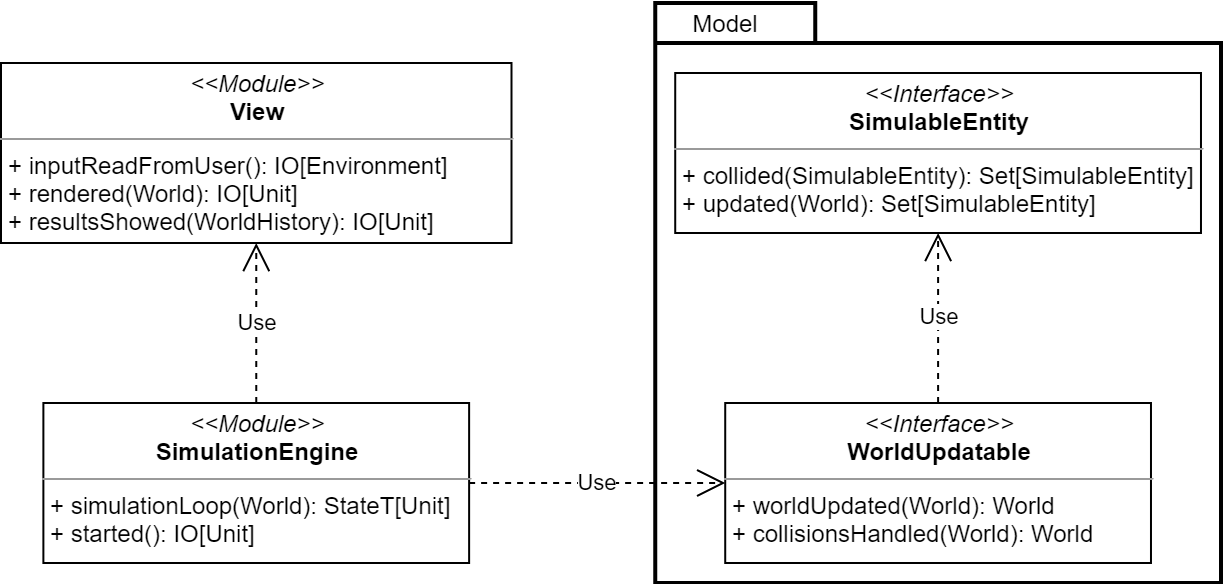
\includegraphics[width=\textwidth, scale=0.44]{img/MainArchitecture.png}
\caption{Design architettura principale}
\label{fig:mainarchitecture}
\end{figure}

\subsection{Pattern MVC}
Come mostrato in Figura \ref{fig:mainarchitecture} le componenti sono interamente indipendenti tra di loro, permettendo una buona separazione delle responsabilità fra le stesse.

\begin{itemize}
    \item Il model interpreta il comportamento dell’applicazione in termini di dominio del problema, in maniera del tutto indipendente dall’interfaccia utente. Il modello gestisce quindi i dati, la logica e le regole dell’applicazione.
    \item Il controller si occupa principalmente di eseguire ed applicare la logica di gioco e di aspetti di interazione tra model e view.
    \item La view visualizza i dati contenuti nel model secondo una rappresentazione testuale o grafica e si occupa dell'interazione tra il simulatore e gli utenti.
\end{itemize}

La separazione dei compiti e dei componenti proposta dall'approccio MVC favorisce il riuso del codice, un aumento della produttività, facilita la manutenzione del software e ne agevola la scalabilità. Nello specifico i vantaggi sono i seguenti:
\begin{itemize}
    \item Esiste la possibilità di scrivere view e controller diversi, utilizzando lo stesso model e quindi, come già accennato, riutilizzare parte del codice scritto in precedenza.
    \item L'utilizzo di un modello rigido e di regole standard nella stesura del progetto facilita un eventuale lavoro di manutenzione e agevola la comprensione anche da parte di altri programmatori esterni.
    \item La possibilità di avere un controllore separato dal resto dell’applicazione, rende la progettazione più semplice e permette di concentrare gli sforzi sulla logica del funzionamento.
    \item Un cambiamento ad un componente generalmente non comporta alcuna modifica necessaria agli altri componenti.
\end{itemize}
